\documentclass{article}
\usepackage[paperwidth=9in, paperheight=11in, margin=12mm]{geometry}
\usepackage{hyperref}

\usepackage{tikz}
\usepackage[]{pgf-umlcd}

\renewcommand{\familydefault}{\ttdefault}

\begin{document}

\section{UML}

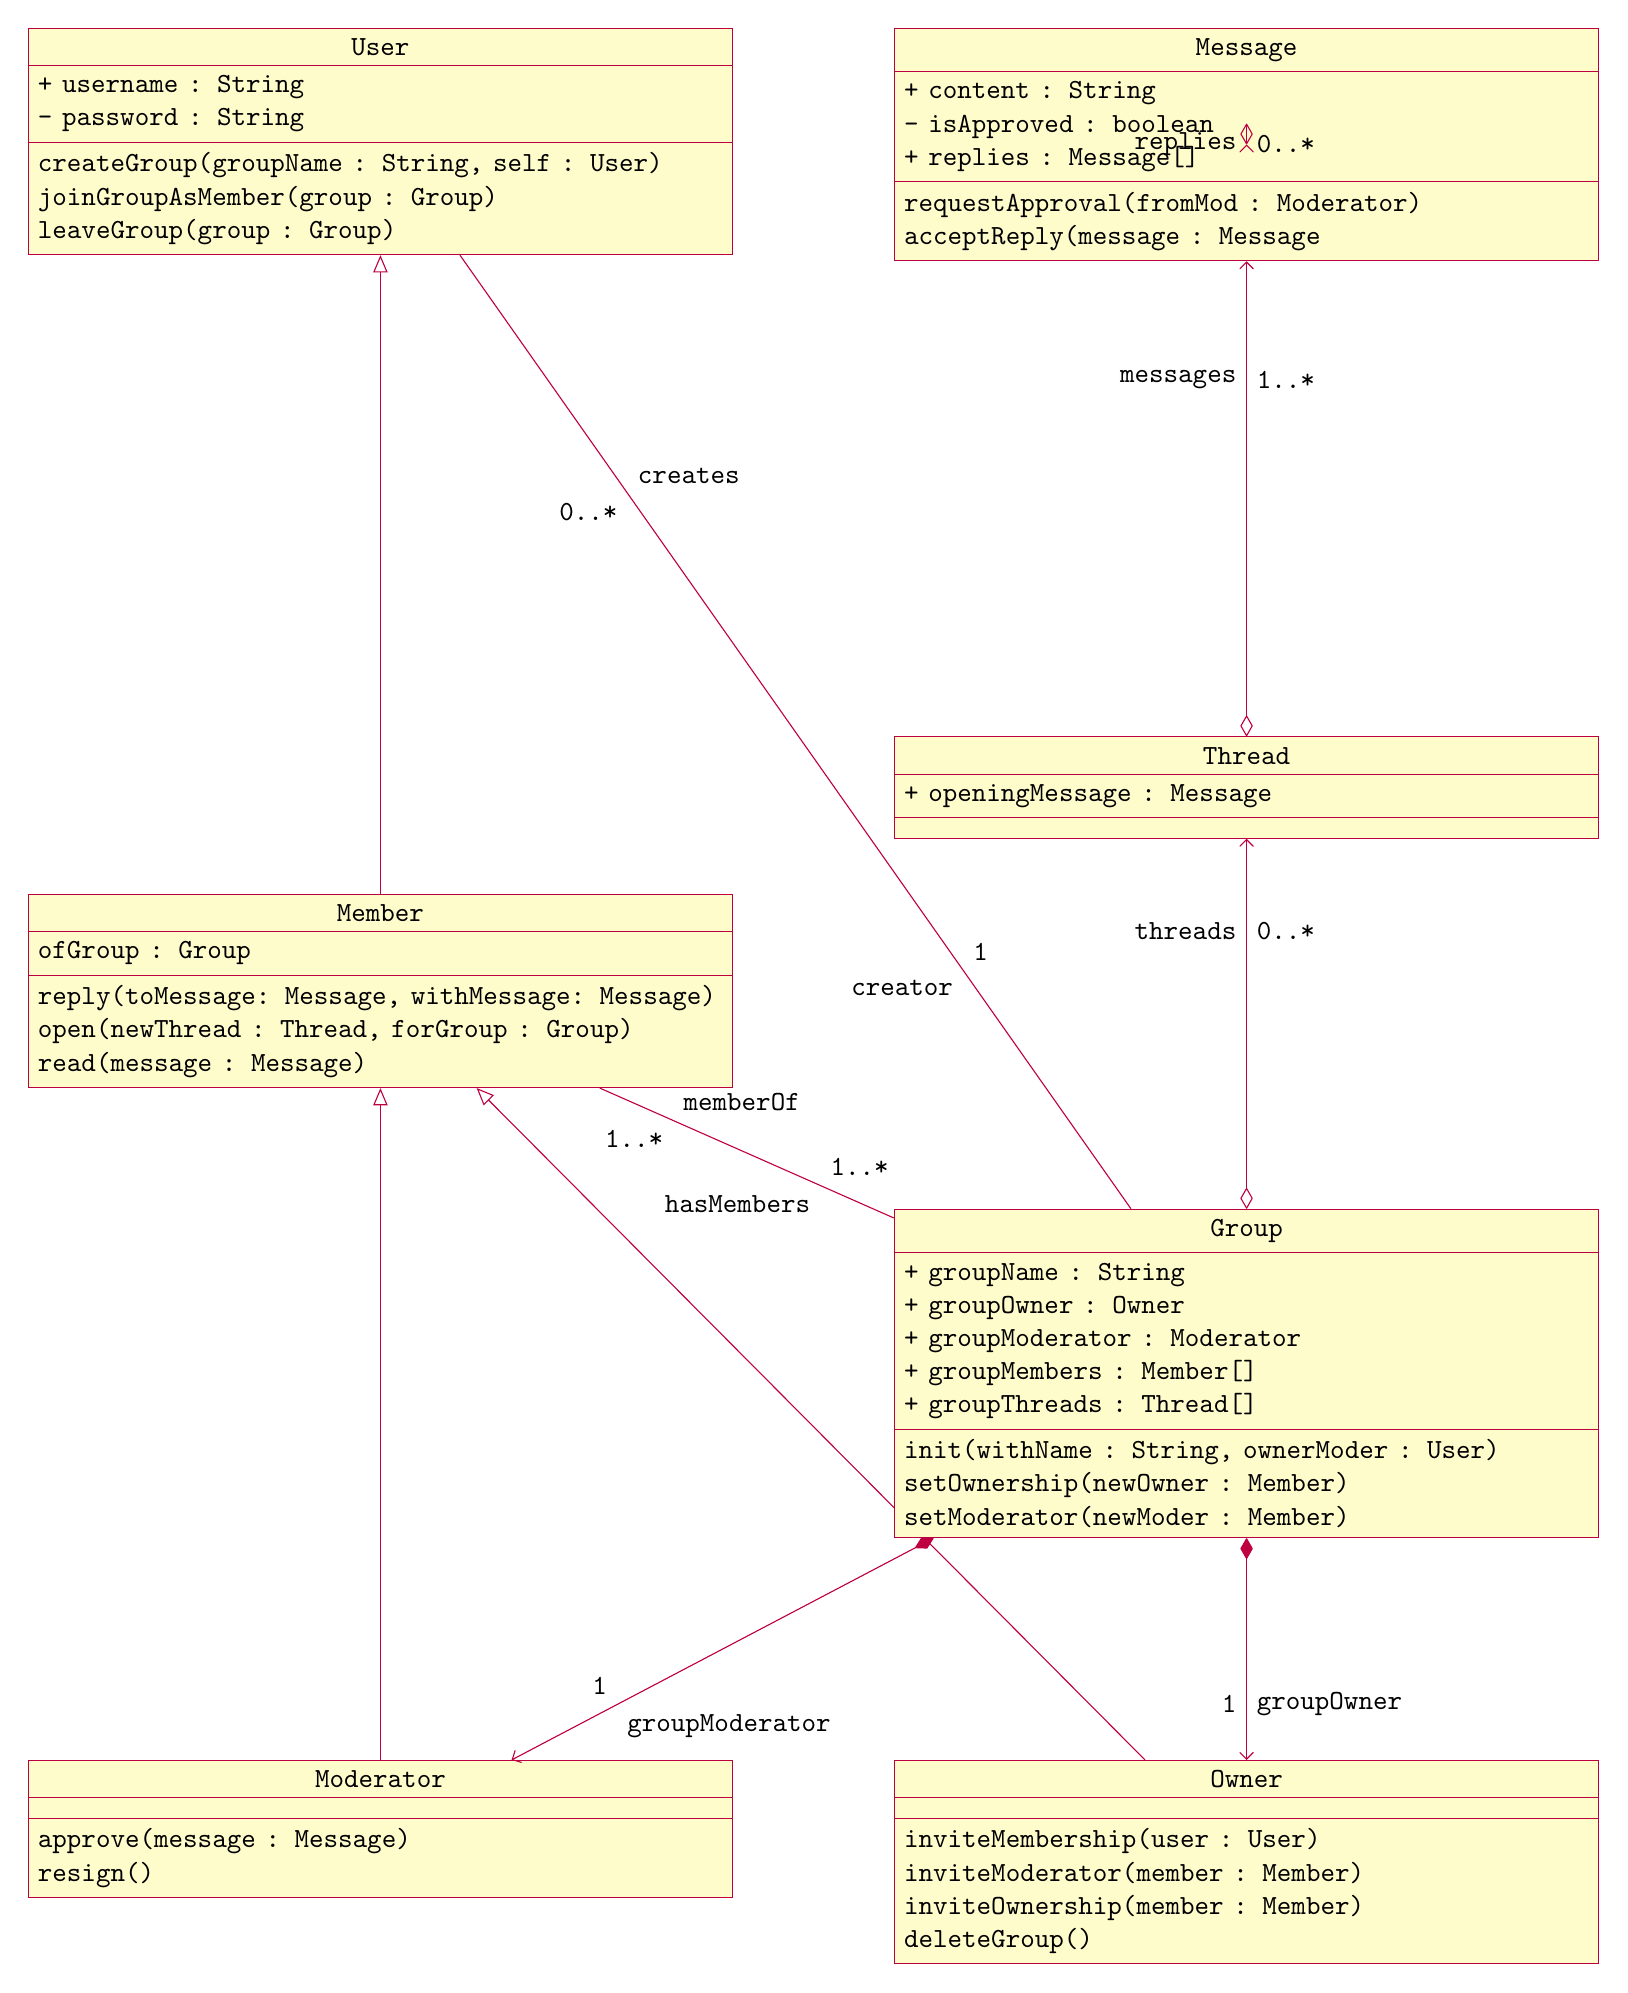
\begin{tikzpicture}%[show background grid]

	\begin{class}[text width=8.7cm]{Group}{11,12}
	
		\attribute{+ groupName : String}
		\attribute{+ groupOwner : Owner}
		\attribute{+ groupModerator : Moderator}
		\attribute{+ groupMembers : Member[]}
		\attribute{+ groupThreads : Thread[]}
		\operation{init(withName : String, ownerModer : User)}
		\operation{setOwnership(newOwner : Member)}
		\operation{setModerator(newModer : Member)}
	    
	\end{class}
	
	\begin{class}[text width=8.7cm]{User}{0,27}
	
		\operation{createGroup(groupName : String, self : User)}
		\operation{joinGroupAsMember(group : Group)}
		\operation{leaveGroup(group : Group)}
		
		\attribute{+ username : String}
		\attribute{- password : String}
	    
	\end{class}
	
	\begin{class}[text width=8.7cm]{Member}{0,16}
	
		\inherit{User}
		
		\attribute{ofGroup : Group}
		
		\operation{reply(toMessage: Message, withMessage: Message)}
		\operation{open(newThread : Thread, forGroup : Group)}
		\operation{read(message : Message)}
	    
	\end{class}
	
	\begin{class}[text width=8.7cm]{Message}{11,27}
	
		\attribute{+ content : String}
		\attribute{- isApproved : boolean}
		\attribute{+ replies : Message[]}
		
		\operation{requestApproval(fromMod : Moderator)}
		\operation{acceptReply(message : Message}
	    
	\end{class}
	
	
	\begin{class}[text width=8.7cm]{Thread}{11,18}
	
		\attribute{+ openingMessage : Message}
	    
	\end{class}
	
	\begin{class}[text width=8.7cm]{Moderator}{0,5}
	
		\inherit{Member}
		
		\operation{approve(message : Message)}
		\operation{resign()}
	    
	\end{class}
	
	\begin{class}[text width=8.7cm]{Owner}{11,5}
	
		\inherit{Member}
		
		\operation{inviteMembership(user : User)}
		\operation{inviteModerator(member : Member)}
		\operation{inviteOwnership(member : Member)}
		\operation{deleteGroup()}
	    
	\end{class}
	
	\composition{Group}{groupOwner}{1}{Owner}
	\composition{Group}{groupModerator}{1}{Moderator}
	\association{User}{creates}{0..*}{Group}{1}{creator}
	\association{Member}{memberOf}{1..*}{Group}{1..*}{hasMembers}
	\aggregation{Thread}{messages}{1..*}{Message}
	\aggregation{Message}{replies}{0..*}{Message}
	\aggregation{Group}{threads}{0..*}{Thread}
	
\end{tikzpicture}

\section{Supplement}

\begin{table}[h]
\begin{center}

	\begin{tabular}{|l|l|}
	\hline
	{\large Relationship} & {\large Data Structures}\\ \hline
	Group to Owner & Group has a reference to owner \\
	Group to Moderator & Group has a reference to moderator \\
	User creating Group & User passes self (this) to init a group, giving reference for owner/moderator. \\
	Members to Group & Group has a hash table of users, used to confirm membership for posting \\
	Threads to Message & Thread has an array of messages, because order matters and the primary operation is printing. \\
	Message to Message & Each Message, as the primary attribute of threads, contains the array of responses to it. \\
	Group to Thread & Likewise, each group contains an ordered array of Threads. \\
	\hline
	\end{tabular}
\end{center}
\end{table}

\end{document}